\chapter{Gaussiane Multivariate}
In questo capitolo estenderemo il concetto di variabile aleatoria gaussiana al caso
multidimensionale, introducendo le \textbf{variabili gaussiane multivariate} o
\textbf{vettori aleatori gaussiani}. Si tratta di vettori casuali la cui distribuzione congiunta è di tipo normale.

\medskip
Le gaussiane multivariate rappresentano una classe di modelli di importanza
fondamentale sia dal punto di vista teorico sia applicativo.  
Da un lato, esse costituiscono il naturale prolungamento della distribuzione
normale univariata, conservandone la struttura analitica e le principali proprietà;
dall’altro, sono ampiamente utilizzate in statistica, in machine learning e nella
modellizzazione di fenomeni multidimensionali di tipo lineare, in quanto completamente
descritte da un vettore di media e da una matrice di covarianza.\\
\\
Nel seguito analizzeremo in dettaglio la loro definizione, le principali
proprietà, la forma della densità, la funzione caratteristica e il ruolo della
matrice di covarianza nella determinazione della dipendenza tra le componenti.\\
\\
Iniziamo ricordando che, data una matrice $C$ simmetrica ($C=C^\top$) e reale, allora esiste una matrice $O$ ortogonale ($O^\top = O^{-1}$) tale che:
\[C = ODO^\top\qquad \text{con $D$ diagonale.}\]

Definiamo ora quando una variabile si dice Gaussiana, senza passare dalla densità, ma utilizzando la funzione caratteristica.

\begin{definizione}[Variabile Gaussiana]
    $X$ è una Variabile Aleatoria Gaussiana se la sua funzione caratteristica è tale che:
    \[\varphi_X(u) = e^{iu\mu}e^{-\frac{\sigma^2 u^2}{2}}\]
\end{definizione}

Siccome $\varphi_X$ caratterizza univocamente una probabilità, allora di conseguenza si ha che, per una variabile aleatoria gaussiana vale che
\[f_X(x) = \frac{1}{\sqrt{2\pi\sigma^2}}e^{-\frac{1}{2}\frac{(x-\mu)^2}{\sigma^2}}\]

È evidente che le due definizioni di variabile aleatoria gaussiana (a partire dalla sua funzione caratteristica, o dalla sua funzione di densità) sono equivalenti. Tuttavia, grazie alla definizione attraverso $\varphi_X$, possiamo includere nelle famiglia delle gaussiane anche il caso degenere in cui $X$ sia una costante; infatti, se $\sigma^2 = 0$, allora $f_X$ esplode, mentre $\varphi_X$ non ha problemi.

\begin{definizione}[Vettore Gaussiano]
\label{def:13.1}
    Sia $\ve{X}:(\Omega, \mathcal{A}, \mathbb{P})\to (\mathbb{R}^n, \mathcal{B}^n)$ un vettore aleatorio. Si dirà che $\ve{X}$ è un Vettore Aleatorio Gaussiano di parametri
    \[\ve{\mu}=\begin{bmatrix}\mu_1\\\vdots\\\mu_n\end{bmatrix}\in\mathbb{R}^n\qquad \text{e}\qquad C = (C_{ij})_{i, j=1, ..., n}\in S^+(n)\]
    se:
    \[\varphi_{\ve{X}} (\ve{u}) = \ex{i\scalar{\mu}{u}-\frac{1}{2}\left\langle\ve{u}, C\ve{u}\right\rangle}\]
    \noindent Dove $S^+(n)$ rappresenta lo spazio delle matrici $n\times n$ simmetriche e semidefinite positive. \footnotetext{Si noti che $\left\langle\ve{u}, C\ve{u}\right\rangle$ è una forma quadratica.}
\end{definizione}

\begin{proposizione}
    $\forall\ve{\mu}\in\mathbb{R}^n\;$ e $\;C\in S^+(n) \;$ esiste un vettore aleatorio $\ve{X}\in\mathbb{R}^n\;$ tale che:
    \[\varphi_{\ve{X}} (\ve{u}) = \ex{i\scalar{\mu}{u}-\frac{1}{2}\left\langle\ve{u}, C\ve{u}\right\rangle}\]
    \begin{dimostrazione}
        Per dimostrare la proposizione procederemo in due fasi, prima analizzando il caso semplice in cui $C$ sia diagonale, e poi il caso generale.\\
        \\
        Se $C$ è diagonale, possiamo definirla come\footnote{Si presti attenzione che i $\sigma_k^2$ non sono ``ancora'' le varianze, ma sono semplicemente i nomi con cui chiamiamo gli elementi di $C$}:
        \[
        C := 
        \begin{bmatrix}
        \sigma_1^2 & 0 & \cdots & 0\\
        0 & \ddots & & \vdots\\
        \vdots & & \ddots & 0\\
        0 & \cdots & 0 & \sigma_n^2
        \end{bmatrix}\qquad \text{con}\qquad \sigma_k^2\geq0\;\;\forall k = 1, ..., n
        \]
        Definiamo inoltre $\ve{\mu} := \begin{bmatrix}\mu_1\\\vdots\\\mu_n\end{bmatrix}.\;$ Consideriamo ora $X_k\overset{\text{i.i.d.}}{\sim}\mathcal{N}(\mu_k, \sigma_k^2)$, e costruiamo $\ve{X}:=\begin{bmatrix}X_1\\\vdots\\X_n\end{bmatrix}$. Siccome le $X_k$ sono indipendenti:
        \begin{align*}
            \varphi_{\ve{X}}(\ve{u}) & = \varphi_{\ve{X}}(u_1, ..., u_n) = \varphi_{X_1}(u_1)\cdots \varphi_{X_n}(u_n) = \ex{iu_1\mu_1 - \frac{1}{2} u_1^2\sigma_1^2} \cdots \ex{iu_n\mu_n - \frac{1}{2} u_n^2\sigma_n^2} \\
            & = \ex{i \sum_{k=1}^n u_k \mu_k - \frac{1}{2}\sum_{k=1}^n u_k^2 \sigma_k^2} = \ex{i\scalar{\mu}{u}-\frac{1}{2}\left\langle\ve{u}, C\ve{u}\right\rangle}
        \end{align*}
        \noindent Che è il vettore gaussiano\\
        \\
        Nel caso generale invece, sapendo che $C=ODO^\top$, con $D$ matrice diagonale, che definiamo esattamente come abbiamo definito $C$ nel punto precedente. Allora (grazie al punto precedente) sappiamo che esiste $\ve{Y}\sim\mathcal{N}(\ve{0}, D)$ vettore gaussiano, dove
        \[\varphi_{\ve{Y}}(\ve{u}) = \ex{-\frac{1}{2}\left\langle\ve{u}, D\ve{u}\right\rangle}\]
        Poniamo $\ve{X}= O\ve{Y} + \ve{\mu}$, allora avremo che (Teorema \ref{th:12.4}):
        \begin{align*}
            \varphi_{\ve{X}}(\ve{u}) & = \ex{i\scalar{\mu}{u}} \cdot \varphi_{\ve{Y}}(O^\top \ve{u}) = \ex{i\scalar{\mu}{u}} \cdot \ex{-\frac{1}{2}\left\langle O^\top \ve{u}, DO^\top \ve{u}\right\rangle} \\
            & = \ex{i\scalar{\mu}{u} - \frac{1}{2}\left\langle \ve{u}, \underbrace{ODO^\top}_C \ve{u}\right\rangle}
        \end{align*}
    \end{dimostrazione}
\end{proposizione}

\begin{definizione}
    $\ve{Z}$ è un vettore gaussiano standard $n$--dimensionale se:
    \[\ve{Z}\sim\mathcal{N}(\ve{0}, I_{n\times n})\qquad \text{ossia con:}\qquad \ve{\mu} = \ve{0}\quad \text{e}\quad C = I_{n\times n}\]
\end{definizione}

\noindent Si osservi che, nel caso in cui $C\in S^+(n)$ allora possiamo scriverla come 
\[
    C = ODO^\top = \underbrace{O \sqrt{D}}_{\sqrt{C}} \;\underbrace{\sqrt{D}O^\top}_{\sqrt{C^\top}} = \sqrt{C}\sqrt{C}^\top
\]
Allora, come facevamo nel caso unidimensionale, è possibile standardizzare un vettore aleatorio gaussiano $\ve{X}\sim \mathcal{N}(\ve{\mu}, C)$, tramite \(\;\ve{X}\sim \sqrt{C} \ve{Z} + \ve{\mu}\). Purtroppo questa non risulta essere un'uguaglianza (come lo era nel caso unidimensionale) puntuale tra i due membri, ma esprime solo che i due vettori hanno la stessa legge\footnote{Le uguaglianze in legge verranno approfondite nei capitoli successivi, si rimanda a quelli per approfondimenti}.

\begin{proposizione}[Proprietà di un Vettore Gaussiano]
\label{prop:13.5}
    Sia $\ve{X}\sim \mathcal{N}(\ve{\mu}, C)$ con $\mu\in\mathbb{R}^n, \;C\in S^+(n)$. Allora:
    \begin{enumerate}
        \item $\E{\ve{X}} = \ve{\mu}\qquad \text{e}\qquad Var(\ve{X}) = C$
        \item $X_k \sim \mathcal{N}(\mu_k, C_{kk})$
        \item Se $\ve{Y} = A\ve{X} + \ve{b}$ con $A\in M(k\times n)$ e $\ve{b}\in\mathbb{R}^k\quad \Rightarrow\quad \ve{Y}\sim \mathcal{N}(A\ve{\mu}+\ve{b}, ACA^\top)$
        \item $X_1, ..., X_n$ sono V.A. indipendenti $\quad \iff \quad Cov(X_i, X_j) = 0 \;\;\forall i\neq j\quad \iff \quad C\;$ è diagonale
    \end{enumerate}
    \begin{dimostrazione}
        1. Sia $\ve{X}\sim \sqrt{C} \ve{Z} + \ve{\mu}$ con $\ve{Z}\sim \mathcal{N}(0, 1)$, allora:
        \begin{align*}
            & \E{\ve{X}} = \sqrt{C}\E{\ve{X}} + \ve{\mu} = \ve{\mu}\\
            & C_{\ve{X}} = E\left[\bigl(\ve{X}-E[\ve{X}]\bigr)\cdot (\ve{X}-E[\ve{X}]\bigr)^\top\right] = \E{\sqrt{C}\ve{Z}\ve{Z}^\top \sqrt{C}^\top} = \sqrt{C} C_{\ve{Z}} \sqrt{C}^\top = \sqrt{C}I\sqrt{C}^\top = C 
        \end{align*}
        2. Dall'applicazione vista a pagina \pageref{pag:107}, con $\ve{v} = [0, ..., u_k, ...0]$:
        \begin{align*}
            \varphi_{X_k}(u_k) = \varphi_{\ve{X}}(\ve{v}) = \ex{i\scalar{\mu}{v}-\frac{1}{2}\left\langle\ve{u}, C\ve{v}\right\rangle} = \ex{i u_k\mu_k -\frac{1}{2}u_k^2C_{kk}} \; \Rightarrow \; X_k\sim\mathcal{N}(\mu_k, C_{kk})
        \end{align*}
        3. Sia $\ve{v}\in \mathbb{R}^k$ (non ci si confonda, non è lo stesso del punto precedente!), allora:
        \begin{align*}
            \varphi_{X_k}(u_k) \overset{\ref{th:12.4}}{=} &e^{i\scalar{v}{b}}\cdot \varphi_{\ve{X}}(A^\top \ve{v}) = e^{i\scalar{v}{b}}\cdot \ex{i \left\langle\ve{\mu}, A^\top\ve{v}\right\rangle -\frac{1}{2} \left\langle A^\top\ve{v}, C_{\ve{X}}A^\top\ve{v}\right\rangle} \\
            = & \ex{i \left\langle\ve{u}, A\ve{\mu}+\ve{b}\right\rangle -\frac{1}{2} \left\langle A^\top \ve{v}, AC_{\ve{X}}A^\top\ve{v}\right\rangle}
        \end{align*}
        4. L'implicazione ($\Rightarrow$) è triviale. Per quanto riguarda l'implicazione ($\Leftarrow$), data $C = \text{diag}(\sigma_1^2, ..., \sigma_n^2)$ si ha che:
        \begin{align*}
        \varphi_{\ve{X}} (\ve{u}) & = \ex{i\scalar{\mu}{u}-\frac{1}{2}\left\langle\ve{u}, C_{\ve{X}}\ve{u}\right\rangle} = \ex{i\sum_{k=1}^n \mu_k u_k - \frac{1}{2}\sum_{k=1}^n u_k\sigma_k^2 u_k} \\
        & = e^{iu_1\mu_1 - \frac{1}{2} u_1^2 \sigma_1^2}\cdots e^{iu_n\mu_n- \frac{1}{2} u_n^2 \sigma_n^2} = \varphi_{X_1}\cdots\varphi_{X_n}
        \end{align*}
    \end{dimostrazione}
\end{proposizione}

Grazie alle proprietà appena illustrate, si evince che dato un vettore gaussiano $\ve{X}$, allora \textbf{ogni suo sottovettore è ancora gaussiano}. Infatti $\exists A\in M(n\times n)$ tale che:
\[\ve{Y}  = A\ve{X} + \ve{b}\sim \mathcal{N}(A\ve{\mu}, AC_{\ve{X}}A^\top)\]

\begin{esempio}
    Si consideri il vettore gaussiano $\ve{X} = [X_1, X_2, X_3]^\top$ come segue:
\[\ve{X}\sim\mathcal{N}\left(\begin{bmatrix} 1\\1\\1\end{bmatrix}, \begin{bmatrix}
    2 & 1 & 0\\
    1 & 1 & 0\\
    0 & 0 & 1
\end{bmatrix}\right)\]
E si prenda il sottovettore $\ve{Y} = [X_1, X_3]^\top$. Allora possiamo vedere $\ve{Y}$ come la trosformazione affine di $\ve{X}$:
\[\ve{Y} = \begin{bmatrix}
    1 & 0 & 0\\
    1 & 0 & 1\\
    \end{bmatrix} \begin{bmatrix} X_1\\X_2\\X_3 \end{bmatrix} \quad \Rightarrow \quad \ve{Y}\sim \left(\begin{bmatrix}1\\1\end{bmatrix}, \begin{bmatrix}
    2 & 0 \\
    0 & 1 \\
    \end{bmatrix}\right)\]
\end{esempio}

Dall'ultimo esempio notiamo un'altra caratteristica riguardanti le componenti di un vettore gaussiano: se ho degli zeri nella matrice di covarianza di un vettore gaussiano, allora vuol dire che le corrispettive componenti sono indipendenti. Dato quindi $\ve{X}\sim \mathcal{N}(\ve{\mu}_{\ve{X}}, C_{\ve{X}})$:
\[X_i \ind X_j \quad \iff \quad C_{ij} = 0\]

\bigskip
\noindent \faWarning $\;$ Si faccia attenzione a non leggere in maniera errata la 2. del precedente teorema: è valida solo in un senso! Infatti, date $X_1, ..., X_n$ variabili aleatorie gaussiane, allora non è detto in generale che il vettore $\ve{X} = [X_1, ..., X_n]^\top$ sia congiuntamente un vettore gaussiano. Questo è valido solo nel caso in cui $X_1, ..., X_n$ sia una famiglia di variabili aleatorie indipendenti, e lo esponiamo nella seguente proposizione.

\bigskip
\begin{proposizione}
\label{prop:13.6}
    \[\begin{aligned}
        &X_1, ..., X_n\\
        \text{ sono indi}&\text{pendenti e gaussiani }
    \end{aligned}\quad \iff \quad \ve{X} = \begin{bmatrix} X_1\\\vdots\\X_n \end{bmatrix} \sim \mathcal{N}(\ve{\mu}, C)\]
    Con $\quad \ve{\mu}_{\ve{X}} = \begin{bmatrix}\ve{\mu}_1\\\ve{\mu}_2\end{bmatrix};\quad C_{\ve{X}} = \begin{bmatrix}\sigma_1^2 & & 0\\
     & \ddots & \\
     0 & & \sigma_n^2
    \end{bmatrix}$

    \bigskip
    \noindent Che può anche essere letto in chiave vettoriale.

    \medskip
    \noindent Siano $\ve{X}_1\sim\mathcal{N}(\ve{\mu_1}, C_1),\;\ve{X}_1\in\mathbb{R}^{n_1}\;\quad \ve{X}_2\sim\mathcal{N}(\ve{\mu_2}, C_2),\;\ve{X}_2\in\mathbb{R}^{n_2}$, e si definisca $\ve{X} = \begin{bmatrix}\ve{X}_1\\\ve{X}_2\end{bmatrix} \in\mathbb{R}^{n_1+n_2}$, allora:
    \[\ve{X}_1 \ind \ve{X}_2\quad \iff \quad \ve{X}\sim\mathcal{N}(\ve{\mu}_{\ve{X}}, C_{\ve{X}})\quad \text{con}\quad \ve{\mu}_{\ve{X}} = \begin{bmatrix}\ve{\mu}_1\\\ve{\mu}_2\end{bmatrix};\quad \text{$C_{\ve{X}}$ a blocchi:}\quad C_{\ve X}=\left[\begin{array}{c|c}
C_1 & 0 \\
\hline
0 & C_2
\end{array}\right]
\]
\end{proposizione}

Unendo il punto 3. della Proposizione \ref{prop:13.5} e la Proposizione \ref{prop:13.6} possiamo osservare che una qualsiasi combinazione lineare di variabili aleatorie gaussiane indipendenti, genera una variabile aleatoria a sua volta gaussiana, ossia: 

\medskip
Siano $X_1\sim\mathcal{N}(\mu_1, \sigma_1^2),\; X_2\sim\mathcal{N}(\mu_2, \sigma_2^2),\;$ tali che $X_1 \ind X_2$:
\[\Rightarrow\quad\forall \alpha, \beta, \gamma\in \mathbb{R}\qquad \alpha X_1 + \beta X_2 + \gamma \sim \mathcal{N}(\alpha \mu_1 + \beta \mu_2 + \gamma, \alpha^2\sigma_1^2 + \beta^2\sigma_2^2)\]

\begin{teorema}
    Sia $\ve{X}\sim \mathcal{N}(\ve{\mu}, C_{\ve{X}})$ con $\ve{\mu}\in\mathbb{R}^n, \;C\in S^+(n), \;$ allora:
    \[\boxed{\ve{X} \;\text{ è assolutamente continuo}\quad \iff \quad \det(C_{\ve{X}})\neq 0} \quad \small\text{(ossia $C_{\ve{X}}$ invertibile)}\]
    E in tal caso ha densità continua:
    \[f_{\ve{X}}(x_1, ..., x_n) = \frac{1}{\sqrt{(2\pi)^{n}\det(C_{\ve{X}})}} \ex{-\frac{1}{2}\left\langle \ve{x}-\ve{\mu}, C^{-1} (\ve{x}-\ve{\mu}) \right\rangle}\]

    \begin{dimostrazione}
        Ricordando che possiamo sempre vedere una gaussiana multivariata $\ve{X}$ come una trasformazione lineare di una gaussiana standard, ossia che $\ve{X} \sim \sqrt{C}\ve{Z} + \ve{\mu}, $ con $\det(\sqrt{C})>0,\; \ve{Z} \sim\mathcal{N}(\ve{0}, I)$. Allora siccome la densità di una normale standard è 
        \[f_{\ve{Z}}(\ve{z}) = \frac{1}{(2\pi)^{n/2}} e^{-\frac{1}{2} ||\ve{z}||^2}\]
        Allora, grazie al punto 2. del riassunto pratico esposto a pagina \ref{riassunto_pratico}, vedendo $\ve{X}$ tramite la trasformazione $h(z) = \sqrt{C}z + \mu \;\Rightarrow\;h^{-1}(x) = \sqrt{C}^{-1}(x-\mu)$, sappiamo che:
        \[f_{\ve{X}}(\ve{x}) = f_{\ve{Z}}(h^{-1}(\ve{x})) \cdot |\det(J_{h^{-1}}(\ve{x}))| = f_{\ve{Z}}\left(\sqrt{C}^{-1}\ve{x}\cdot\right) \frac{1}{\sqrt{\det{C}}}\]
    \end{dimostrazione}
\end{teorema}

Il teorema appena illustrato risponde alla domanda: \textit{abbiamo delle condizioni per verificare se un vettore gaussiano sia assolutamente continuo?}. Questo può essere declinato nella casistica multidimensionale e unidimensionale:
\begin{itemize}
    \item Se $n=1:\quad X\sim \mathcal{N}(\mu, \sigma^2)\quad$ allora:
    \begin{itemize}
        \item Se $\sigma^2 >0 \quad \Rightarrow \quad X$ è assolutamente continua, con densità:
        \[f_X(t) = \frac{1}{\sqrt{2\pi\sigma^2}} e^{-\frac{1}{2}\frac{(t-\mu)^2}{\sigma^2}}\]
        \item Se $\sigma^2 =0 \quad \Rightarrow \quad X \overset{\text{q.c.}}{=}\mu\quad \Rightarrow \quad X$ è discreta e non ammette densità continua.
    \end{itemize}
    \item Se $n>1:\quad \ve{X} \sim \mathcal{N}(\ve{\mu}, C_{\ve{X}})\quad$ allora sappiamo che $\ve{X}\in \text{Im}(C_{\ve{X}}) + \ve{\mu}$ quasi certamente. Allora:
    \begin{itemize}
        \item Se $\det(C_{\ve{X}}) \neq 0\quad \Rightarrow \quad \ve{X}$ è assolutamente continuo
        \item Se $\det(C_{\ve{X}}) = 0\quad \Rightarrow \quad \ve{X}$ non è assolutamente continuo. 

        \medskip 
        \noindent Questo vuol dire che esiste sicuramente un vettore $\;\ve{a}\neq \ve{0}\;$ tale che $\;\ve{a} \in \ker(C_{\ve{X}}),\;$ ossia che $C\ve{a} = \ve{0}$. Questo implica che la varianza lungo la direzione $\;\ve{a}\;$ è zero. Ciò significa che $\ve{X}$ vive interamente su un \textit{sottospazio affine} di dimensione $n-1$
        \[H = \set{\ve{x}\in\mathbb{R}^n\mid \left\langle\ve{x} - \ve{\mu}, \ve{a}\right\rangle = 0}\]
        $\quad$ siccome la proiezione di $(\ve{X}-\ve{\mu})$ lungo la direzione $\ve{a},\;\left\langle\ve{X} - \ve{\mu}, \ve{a}\right\rangle$, è uguale a zero quasi certamente. $\ve{X}$ non si muove lungo la direzione $\ve{a}$.  
    \end{itemize}
\end{itemize}

\begin{esempio}
    Si consideri il vettore gaussiano $\ve{X} = [X_1, X_2]^\top$:
    \[\ve{X}\sim\mathcal{N}\left(\begin{bmatrix} 1\\1\end{bmatrix}, \begin{bmatrix}
    1 & 1 \\
    1 & 1 \\
\end{bmatrix}\right);\qquad A = \set{(x_1, x_2)\in\mathbb{R}^2\mid x_1^2+x_2^2\leq1}\]
Si vuole calcolare $P^{\ve{X}}(A).$

\medskip
\noindent Si nota immediatamente che $\det(C) = 0$. Inoltre si può anche notare che $Cov(X_1, X_2)=1$, implicando che le due componenti abbiamo una relazione deterministica.\\
Si ricava $\ve{a}$ tale che appartenga al $\ker(C)$:
\[C\ve{a} = \ve{0} \quad \Rightarrow \quad \ve{a} = [a_1, -a_1]^\top\]

Quindi $\ve{X}$ vive sul sottospazio affine tale che la sua proiezione lungo $\ve{a}$ sia uguale a zero:
\[\left\langle\ve{X} - \ve{\mu}, \ve{a}\right\rangle = 0 \quad \Rightarrow \quad X_1=X_2\]
Ossia che vive sul sottospazio:
\[H = \set{(x_1, x_2)\in\mathbb{R}^2\mid x_1=x_2}\]

Allora il calcolo della probabilità diventa, definendo $X_1 = X_2 =: Y$:
\[P^{\ve{X}}(A) = \mathbb{P}(\ve{X}\in A) = \mathbb{P}\left(-\frac{1}{\sqrt{2}}\leq Y\leq \frac{1}{\sqrt{2}}\right) = \Phi\left(\frac{1}{\sqrt{2}}-1\right) - \Phi\left(-\frac{1}{\sqrt{2}}-1\right) \simeq 0.3409\]

In quanto $C$ è il cerchio di raggio $1$ centrato in $0$, e $\ve{X}$ vive sulla retta $x_1=x_2$.

\begin{figure}[H]
\centering
\begin{tikzpicture}[scale=2, >=stealth, font=\small]
  % --- Assi ---
  \draw[->] (-1.3,0) -- (1.3,0) node[right] {$x_1$};
  \draw[->] (0,-1.3) -- (0,1.3) node[above] {$x_2$};

  % --- Cerchio unitario ---
  \fill[blue!8] (0,0) circle (1);
  \draw[blue, thick] (0,0) circle (1) node[below=5pt, right=2pt] {$x_1^2 + x_2^2 = 1$};

  % --- Retta x1 = x2 ---
  \draw[gray, dashed] (-1.2,-1.2) -- (1.2,1.2) node[above right] {$x_1 = x_2$};

  % --- Segmento all'interno del cerchio ---
  \coordinate (A) at ({-1/sqrt(2)},{-1/sqrt(2)});
  \coordinate (B) at ({ 1/sqrt(2)},{ 1/sqrt(2)});
  \draw[red, very thick] (A) -- (B);

  % --- Estremi e origine ---
  \fill[red] (A) circle (0.02) node[below left] {$\big(-\tfrac{1}{\sqrt2},-\tfrac{1}{\sqrt2}\big)$};
  \fill[red] (B) circle (0.02) node[above right] {$\big(\tfrac{1}{\sqrt2},\tfrac{1}{\sqrt2}\big)$};
  \fill (0,0) circle (0.02);
\end{tikzpicture}

\label{fig:gaussiana_degenere_cerchio}
\end{figure}




\end{esempio}

Dall'esempio abbiamo quindi appurato che un vettore può essere gaussiano anche se non è assolutamente continuo, e in questo caso si definisce \textit{Gaussiano Degenere}. Infatti, nella definizione \ref{def:13.1} non si accenna ad assoluta continuità, ma si definisce gaussiano un qualsiasi vettore che abbia quella funzione caratteristica.